\section{Aplicaciones económicas}

\begin{frame}[t]
\frametitle{\secname}

\begin{theorem}[Igualdad de las derivadas cruzadas o teorema de Schwarz]
Supnga que todas $m$--ésimas derivadas parciales de una función $f\left(x_{1},\ldots,x_{n}\right)$ son continuas. Si cualquiera dos de ellas involucran diferenciación con respecto a cada una de las variables el mismo número de veces, entonces ellas son necesariamente iguales.
\end{theorem}

El contenido de este resultado puede ser explicado como sigue: Sea $m=m_{1}+\cdots+m_{n}$ y suponga que $f\left(x_{1},x_{2},\ldots,x_{n}\right)$ es diferenciable $m_{1}$ veces con respecto a $x_{1}$, $m_{2}$ veces diferenciable con respecto a $x_{2}$, \ldots, y $m_{n}$ veces diferenciable con respecto a $x_{n}$. Suponga que la condición de continuidad es satisfecha por estas derivadas parciales de orden $m$--ésimo. Entonces terminamos con el mismo resultado sin importar cuál sea el orden de la diferenciación, porque cada una de las derivadas parciales es igual a \[ \frac{\partial^{m}f}{\partial x^{m_{1}}_{1}\partial x^{m_{2}}_{2}\cdots\partial x^{m_{n}}_{n}}. \] En particular, para el caso cuando $m=2$, para $i=1,\ldots,n$ y $j=1,\ldots,n$, \[ \frac{\partial^{2}f}{\partial x_{j}\partial x_{i}}=\frac{\partial^{2}f}{\partial x_{i}\partial x_{j}} \] si ambas estas derivadas parciales son continuas.
\end{frame}

\begin{frame}[t]
\frametitle{\secname}

\begin{example}
Considere la función de producción agricultura $Y=F\left(K,L,T\right)$, donde $Y$ es el número de unidades producidas, $K$ es el capital invertido, $L$ es la entrada trabajo y $T$ es el área de tierra agrícola que es usada. Entonces $\partial Y/\partial K=F^{\prime}_{K}$ es llamada el \emph{capital del producto marginal}. Esta es la tasa de cambio de la salida $Y$ con respecto a $K$ cuando $L$ y $T$ se mantienen fijos. Similarmente, $\partial Y/\partial L=F^{\prime}_{L}$ y $\partial Y/\partial T=F^{\prime}_{T}$ son los productos de trabajo y tierra marginales, respectivamente. Por ejemplo, si $K$ es el valor del capital equipado medido en dólares, y $\partial Y/\partial K=5$, entonces aumentar la entrada de capital en $h$ unidades aumentaría la producción en aproximadamente $5h$ unidades.

\

Suponga, en particular, que $F$ es la función de Cobb-Douglas $F\left(K,L,T\right)=AK^{a}L^{b}T^{c}$, donde $A$, $a$, $b$ y $c$ son constantes positivas. Encuentre los productos marginales, y las segundas derivadas parciales. Discuta sus signos.
\end{example}
\end{frame}

\begin{frame}[t]
	\frametitle{\secname}
\begin{proofs}
Los productos marginales son \[ F^{\prime}_{K}=AaK^{a-1}L^{b}T^{c},\quad F^{\prime}_{L}=AbK^{a}L^{b-1}T^{c},\quad\text{y}\quad F^{\prime}_{T}=AcK^{a}L^{b}T^{c-1}. \] Asumiendo que $K$, $L$ y $T$ son todas positivas, los productos marginales son positivos. Por lo tanto, un incremento en el capital, trabajo o tierra incrementará el número de unidades producidas.

Las segundas derivadas parciales cruzadas, también llamadas parciales mixtas son: \[ F^{\prime\prime}_{KL}=AabK^{a-1}L^{b-1}T^{c},\quad F^{\prime\prime}_{KT}=AacK^{a-1}L^{b}T^{c-1},\quad\text{y}\quad F^{\prime\prime}_{LT}=AbcK^{a}L^{b-1}T^{c-1}. \] Note que estas derivadas son positivas. Llamaremos cada par de factores \emph{complementarios} porque más de uno incrementa el producto marginal de la otra.

Las segunda derivadas parciales directas son \[ F^{\prime\prime}_{KK}=Aa\left(a-1\right)K^{a-2}L^{b}T^{c},\quad F^{\prime\prime}_{LL}=Ab\left(b-1\right)K^{a}L^{b-2}T^{c},\quad F^{\prime\prime}_{TT}=Ac\left(c-1\right)K^{a}L^{b}T^{c-2}. \]
\end{proofs}
\end{frame}

\begin{frame}[t]
\frametitle{\secname}
\begin{proofs}[\proofname\ (Cont.)]
Por ejemplo, $F^{\prime\prime}_{KK}$ es la derivada parcial del producto de capital marginal, $F^{\prime}_{K}$ con respecto a $K$.

\

Si $a<1$, entonces $F^{\prime\prime}_{KK}<0$, y existe una disminución del producto del capital marginal, esto es, un pequeño aumento en el capital invertido conducirá a una disminución en el producto marginal del capital.

\

Podemos interpretar que esto significa que, aunque pequeños aumentos de capital porque la producción aumentará, así que $F^{\prime}_{K}>0$, este aumento ocurre en una tasa decreciente, dado que $F^{\prime\prime}_{KK}<0$.

\

Similarmente para el trabajo si $b<1$, y para la tierra si $c<1$.
\end{proofs}
\end{frame}

\subsection{Elasticidades parciales}

\begin{frame}
\frametitle{\subsecname}

\begin{definition}
Si $z=f\left(x,y\right)$, definimos la elasticidad parcial de $z$ con respecto a $x$ e $y$ por
\begin{equation}
\operatorname{El}_{x}z=\frac{x}{z}\frac{\partial z}{\partial x},\quad\operatorname{El}_{y}\left(z\right)=\frac{y}{z}\frac{\partial z}{\partial y}
\end{equation}
\end{definition}

A menudo los economistas solo se refieren a la elasticidad antes que a la elasticidad parcial. Así, $\operatorname{El}_{x}z$ es la elasticidad de $z$ con respecto a $x$ cuando $y$ se mantiene constante, y $\operatorname{El}_{y}z$ tiene su correspondiente interpretación.

Cuando todas las variables son positivas, las elasticidades pueden expresarse como derivadas logarítmicas. De acuerdo
\begin{equation}
\operatorname{El}_{x}z=\frac{\partial\ln z}{\partial\ln x},\quad\text{y}\quad\operatorname{El}_{y}z=\frac{\partial\ln z}{\partial\ln y}.
\end{equation}
\end{frame}

\begin{frame}
	\frametitle{\subsecname}
\begin{definition}
Si $z=f\left(x_{1},x_{2},\ldots,x_{n}\right)=f\left(\bm{x}\right)$, definimos la elasticidad (parcial) de $z$, o de $f$, con respecto a $x_{i}$ como la elasticidad de $z$ con respecto a $x_{i}$ cuando todas las demás variables se mantienen constantes. Así, asumiendo que todas las variables son positivas, podemos escribir
\begin{equation}
\operatorname{El}_{i}z=\frac{x_{i}}{f\left(\bm{x}\right)}\frac{\partial f\left(\bm{x}\right)}{\partial x_{i}}=\frac{x_{i}}{z}\frac{\partial z}{\partial x_{i}}=\frac{\partial\ln z}{\partial\ln x_{i}}.
\end{equation}
\end{definition}

El número $\operatorname{El}_{i}z$ es aproximadamente igual al cambio porcentual en $z$ causado por un $1\%$ de incremento en $x_{i}$, la $i$--ésima variable, manteniendo todas las otras $x_{j}$ constantes. Entre otras formas de notación de uso común en lugar de $\operatorname{El}_{i}z$, mencionamos: $\operatorname{El}_{i}f\left(\bm{x}\right)$, $\operatorname{El}_{x_{i}}z$, $\varepsilon_{i}$, $e_{i}$ y $\hat{z}_{i}$. Este último, por supuesto, se pronuncia ``z sombrero i''.

\end{frame}

\begin{frame}[t]
\frametitle{\subsecname}

\begin{example}
Suponga que $D=Ax^{a_{1}}_{1}x^{a_{2}}_{2}\cdots x^{a_{n}}_{n}$ es definido para todos los $x_{1}>0$, $x_{2}>0$,\ldots,$x_{n}>0$, donde $A>0$ y $a_{1},a_{2},\ldots,a_{n}$ son constantes. Encuentre la elasticidad de $D$ con respecto a $x_{i}$, para $i=1,\ldots,n$.
\end{example}

\begin{proof}
Debido a que todos los factores excepto $x^{a_{i}}_{i}$ son constantes, podemos aplicar la ecuación anterior para obtener el resultado $\operatorname{El}_{i}D=a_{i}$.
\end{proof}

\end{frame}

\begin{frame}[t]
\frametitle{\subsecname}
Como un caso especial de este ejemplo, suponga que $D_{i}=Am^{\alpha}p^{-\beta}_{i}p^{\gamma}_{j}$, donde $m$ es el ingreso, $p_{i}$ es el propio precio y  $p_{j}$ es el precio de un bien sustituto.

\

Entonces, $\alpha$ es la elasticidad ingreso de la demanda. Por otra parte, $-\beta$ es la elasticidad de la demanda con respecto a los cambios en sus propios precios $p_{i}$, por eso se llama \emph{elasticidad de precio propio} de la demanda. Sin embargo, debido a que las elasticidades de demanda del precio propio son generalmente negativas, a menudo se describe $\beta$ antes que $-\beta$ como la elasticidad de la demanda a precio propio.

\

Finalmente, $\gamma$ es la elasticidad de la demanda con respecto al precio del sustituto especificado. Por analogía con las derivadas parciales cruzadas, se llama \emph{elasticidad de precio cruzado} de la demanda. Tenga en cuenta que la proporción del ingreso gastado en bienes es \[ \frac{p_{i}D_{i}}{m}=Am^{\alpha-1}p^{1-\beta}_{i}p^{\gamma}_{j}. \]
\end{frame}

\begin{frame}[t]
\frametitle{\subsecname}
Cuando la elasticidad de ingreso $\alpha<1$, esta proporción es una función de ingreso decreciente. Los economistas describen un producto con esta propiedad como una \emph{necesidad}. Por otro lado, cuando $\alpha>1$, la proporción de ingreso gastado en un producto $i$ aumenta con el ingreso, en cuyo caso los economistas describen el producto $i$ como un lujo.

\begin{remark}
Si $z=f\left(x_{1},\ldots,x_{n}\right)$ es continuamente diferenciable y $x_{i}=g_{i}\left(t_{1},\ldots,t_{m}\right)$, para cada $i=1,2,\ldots,n$ son todas diferenciables, entonces \[ \frac{\partial z}{\partial t_{j}}=\frac{\partial z}{\partial x_{1}}\frac{\partial x_{1}}{\partial t_{j}}+\frac{\partial z}{\partial x_{2}}\frac{\partial x_{2}}{\partial t_{j}}+\cdots+\frac{\partial z}{\partial x_{n}}\frac{\partial x_{n}}{\partial t_{j}} \] para cada $j=1,2,\ldots,m$.
\end{remark}
\end{frame}

\begin{frame}[t]
\frametitle{\subsecname}
Un pequeño cambio en una variable básica $t_{j}$ desencadena una reacción en cadena. En primer lugar, cualquier $x_{i}$ depende de $t_{j}$ en general, por lo que cambia cuando $t_{j}$ ha cambiado. Esto afecta a su vez a $z$. La contribución de la derivada total de $z$ con respecto a $t_{j}$ que resulta de los cambios en $x_{i}$ es $\left(\partial z/\partial x_{i}\right)\left(\partial x_{i}/\partial t_{j}\right)$. La fórmula~\eqref{eq:sumofderivatives} muestra

\begin{equation}\label{eq:sumofderivatives}
F^{\prime}_{j}\left(\bm{t}\right)=f^{\prime}_{1}\left(\bm{x}\right)\frac{\partial g_{1}}{\partial t_{j}}\left(\bm{t}\right)+f^{\prime}_{2}\left(\bm{x}\right)\frac{\partial g_{2}}{\partial t_{j}}\left(\bm{t}\right)+\cdots+f^{\prime}_{n}\left(\bm{x}\right)\frac{\partial g_{n}}{\partial t_{j}}\left(\bm{t}\right).
\end{equation}




\begin{example}
Considere la función de producción agrícola $Y=F\left(K,L,T\right)$, donde $Y$ es el tamaño de la cosecha, $K$ es el capital invertido, $L$ es el trabajo y $T$ es la tierra agrícola utilizada para cultivar. Suponga que $K$, $L$ y $ T$ son todas funciones del tiempo, que es denotado por $t$. Entonces de acuerdo con~\eqref{eq:sumofderivatives}, uno tiene
\[ \dfrac{\mathrm{d}Z}{\mathrm{d}t}=\frac{\partial F}{\partial K}\frac{\mathrm{d}K}{\mathrm{d} t}+\frac{\partial F}{\partial L}\frac{\mathrm{d}L}{\mathrm{d}t}ü\frac{\partial F}{\partial T}\frac{\mathrm{d}T}{\mathrm{d}t}. \]
\end{example}
\end{frame}

\begin{frame}[t]
\frametitle{\subsecname}

\begin{example}
En el caso especial cuando $F$ es la función de Cobb-Douglas $F\left(K,L,T\right)=AK^{a}L^{b}T^{c}$, entonces
\begin{equation}\label{eq:dydt}
\frac{\mathrm{d}Y}{\mathrm{d}t}=aAK^{a-1}L^{b}T^{c}\frac{\mathrm{d}K}{\mathrm{d}t}+bAK^{a}L^{b-1}T^{c}\frac{\mathrm{d}L}{\mathrm{d}t}+cAK^{a}L^{b}T^{c-1}\frac{\mathrm{d}T}{\mathrm{d}t}\notag{*}
\end{equation}
Denotando las derivadas temporales por puntos, y dividiendo cada término en~\eqref{eq:dydt} por $Y=AK^{a}L^{b}T^{c}$, tenemos \[ \frac{\dot{Y}}{Y}=a\frac{\dot{K}}{K}+b\frac{\dot{L}}{L}+c\frac{\dot{T}}{T}. \] La tasa relativa de cambio de la salida es, por lo tanto, la suma ponderada de las tasas relativas del cambio del capital, trabajo y tierra. Los pesos son las respectivas potencias $a$, $b$ y $c$.
\end{example}

\end{frame}

\section{Elasticidad de sustitución}

\begin{frame}[t]
\frametitle{\secname}

Los economistas con frecuencia están interesados en la pendiente de la recta tangente a la curva de nivel en un punto particular. Frecuentemente, la curva de nivel está inclinada hacia abajo, pero los economistas prefieren una respuesta positiva. Así, podemos cambiar el signo de la pendiente, y usar un nombre especial

\begin{definition}[Tasa marginal de sustitución]
\begin{equation}
R_{yx}=\frac{F^{\prime}_{x}\left(x,y\right)}{F^{\prime}_{y}\left(x,y\right)}
\end{equation}
es conocida como la \emph{tasa marginal de sustitución de} $y$ \emph{por} $x$, abreviadamente como \textsc{MRS}.
\end{definition}

\

Note que $R_{yx}=-y^{\prime}\approx-\frac{\Delta y}{\Delta x}$ cuando nos movemos a largo de la curva de nivel $F\left(x,y\right)=c$. Si $\Delta x=-1$ en particular, entonces $R_{yx}\approx\Delta y$. Así, $R_{yx}$ es aproximadamente la cantidad de $y$ podemos agregar por unidad de $x$ removida, si permanecemos en la misma curva de nivel.
\end{frame}

\begin{frame}
\frametitle{\secname}
	\begin{minipage}{0.45\textwidth}
		\begin{example}
		Sea $F\left(K,L\right)=100$ una isocuanta para la función de producción, donde $K$ es la entrada de capital, $L$ es la entrada de trabajo y $100$ es la salida. Vea la figura~\ref{fig:isoquant}.
		En todos los puntos $P$, $Q$ y $R$ se producen $100$ unidades. En $P$ un pequeño capital de entrada y bastante entrada de trabajo son empleados.
		
		\
		
		La pendiente de la isocuanta en $P$ es aproximadamente $-4$, así que el \textsc{MRS} en $P$ es aproximadamente $4$.
		\end{example}
	\end{minipage}
	\begin{minipage}{0.45\textwidth}
		\begin{figure}[ht!]
			\centering
			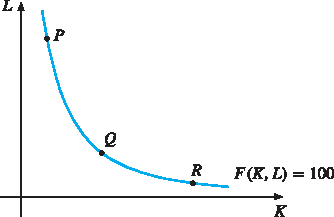
\includegraphics[width=0.4\paperwidth]{isocuant}
			\caption{Una isocuanta.}\label{fig:isoquant}
		\end{figure}
	\end{minipage}
\end{frame}

\begin{frame}[t]
\frametitle{\secname}
Esto significa que para cada cuatro unidades de trabajo que se llevan, agregando solo una unidad de capital nos asegurará que la salida permanece en (aproximadamente) $100$ unidades. Siempre que se elijan unidades para que el capital y el trabajo tengan el mismo precio, el capital en $P$ es más ``valioso'' que el trabajo.

\

En $Q$ el \textsc{MRS} es aproximadamente $1$, así que el capital y el trabajo son igualmente ``valiosos''.

\

Finalmente, en $R$, el \textsc{MRS} es aproximadamente $\frac{1}{5}$, así en este punto aproximadamente cinco unidades de capital son requeridos para compensar la pérdida de una unidad de trabajo.

\

\begin{remark}
Esto nos da una aproximación a la curva $y=f\left(x\right)$ en que la coordenada $y$ de $B$ es una aproximación a la coordenada $y$ de $A$ en la gráfica de $y=f\left(x\right)$.
\end{remark}
\end{frame}

\begin{frame}
\frametitle{\secname}
	\begin{minipage}{0.45\textwidth}
		\begin{example}
		Considere la curva de nivel $F\left(x,y\right)=c$ para la función $F$ de dos variables, como es mostrado en la figura~\ref{fig:RYY} La \textsc{MRS} varía a lo largo de la curva.
		
		\
		
		En el punto $P$, $R_{yx}$ es un número positivo grande. En $Q$, el número $R_{yx}$ es alrededor $1$, y en $R$ este es alrededor de $0.2$. Cuando nos movemos a lo largo de la curva de nivel desde la izquierda hacia la derecha, $R_{yx}$ será estrictamente decreciente con valores en algún intervalo positivo $I$.
		\end{example}
	\end{minipage}
	\begin{minipage}{0.45\textwidth}
		\begin{figure}
			\centering
			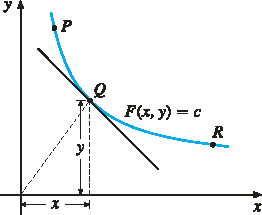
\includegraphics[width=0.4\paperwidth]{ryy}
			\caption{$R_{yy}$ en $Q$.}\label{fig:RYY}
		\end{figure}
	\end{minipage}
\end{frame}

\begin{frame}[t]
\frametitle{\secname}
Para cada valor de $R_{yx}$ en $I$, existe un punto correspondiente $\left(x,y\right)$ en la curva de nivel $F\left(x,y\right)=c$, así un valor correspondiente de $\frac{y}{x}$. La fracción $\frac{y}{x}$ es por lo tanto una función de $R_{zx}$ y se define la siguiente:
\begin{definition}
Cuando $F\left(x,y\right)=c$, la \emph{elasticidad de sustitución entre} $y$ \emph{y} $x$ es \[ \sigma_{yx}=\operatorname{El}_{R_{yx}}\left(\frac{y}{x}\right). \]
\end{definition}

Así, $\sigma_{xy}$ es la elasticidad de sustitución de la fracción $\frac{y}{x}$ con respecto a la \textsc{MRS}. Más o menos, $\sigma_{yx}$ es el porcentaje de cambio en la fracción $\frac{y}{x}$ cuando nos movemos a lo largo de la curva de nivel $F\left(x,y\right)=c$ lo suficientemente lejos para que $R_{yx}$ incremente en un $1\%$.

\begin{remark}
Note que $\sigma_{yx}$ es simétrico en $x$ e $y$. De hecho, $R_{xy}=\frac{1}{R_{yx}}$, así que la fórmula logarítmica para elasticidades implica que $\sigma_{xy}=\sigma_{yx}$.
\end{remark}

\end{frame}

\begin{frame}[t]
\frametitle{\secname}
\begin{example}
Calcule la elasticidad de sustitución $\sigma_{KL}$ de la función Cobb-Douglas $F\left(K,L\right)=AK^{a}L^{b}$.
\end{example}

\begin{proof}
La \textsc{MRS} de $K$ para $L$ es \[ R_{KL}=\frac{F^{\prime}_{L}}{F^{\prime}_{K}}=\frac{bAK^{a}L^{b-1}}{aAK^{a-1}L^{b}}=\frac{b}{a}\frac{K}{L}. \] Por lo tanto, $\frac{K}{L}=\left(\frac{a}{b}\right)R_{KL}$. La elasticidad de la última expresión con respecto a $R_{KL}$ es $1$. Así, $\sigma_{KL}=1$ para la función de Cobb-Douglas.
\end{proof}

\begin{example}
Encuentre la elasticidad de sustitución para la función \textsc{CES} \[ F\left(K,L\right)=A{\left(aK^{-\rho}+bL^{-\rho}\right)}^{-\mu/\rho} \] donde $A$, $a$, $b$, $\mu$ y $\rho$ son constantes, $A>0$, $a>0$, $b>0$, $\mu\neq0$, $\rho>-1$ y $\rho\neq0$.
\end{example}

\end{frame}

\begin{frame}[t]
\frametitle{\secname}
\begin{proofs}
Aquí
\begin{align*}
F^{\prime}_{K}&=A{\left(-\frac{\mu}{\rho}\right)\left(aK^{-\rho}+bL^{-\rho}\right)}^{\left(-\frac{\mu}{\rho}\right)-1}a\left(-\rho\right)K^{-\rho-1},\\
F^{\prime}_{L}&=A{\left(-\frac{\mu}{\rho}\right)\left(aK^{-\rho}+bL^{-\rho}\right)}^{\left(-\frac{\mu}{\rho}\right)-1}b\left(-\rho\right)L^{-\rho-1}.
\end{align*}

Así, \[ R_{KL}=\frac{F^{\prime}_{L}}{F^{\prime}_{K}}=\frac{b}{a}\frac{L^{-\rho-1}}{K^{-\rho-1}}=\frac{b}{a}{\left(\frac{K}{L}\right)}^{\rho+1} \] y por lo tanto \[ \frac{K}{L}={\left(\frac{a}{b}\right)}^{\frac{1}{\left(\rho+1\right)}}{\left(R_{KL}\right)}^{^{\frac{1}{\left(\rho+1\right)}}} \]
\end{proofs}.
\end{frame}

\begin{frame}[t]
\frametitle{\secname}
\begin{proofs}[\proofname\ (Cont.)]
Recordando que la elasticidad de $Ax^{b}$ con respecto a $x$ es $b$, implica que \[ \sigma_{KL}=\operatorname{El}_{R_{KL}}\left(\frac{K}{L}\right)=\frac{1}{\rho+1}. \] Hemos mostrado que la función $F$ tiene elasticidad de sustitución constante $\frac{1}{\left(\rho+1\right)}$. Este, por supuesto, es la razón porqué $F$ es llamada la función \textsc{CES} ``elasticidad de sustitución constante''
\end{proofs}

\

\begin{remark}
Note que la elasticidad de sustitución para la función \textsc{CES} tiende a $1$ cuando $\rho\to0$, el cual es precisamente la elasticidad de sustitución para la función Cobb-Douglas en el ejemplo anterior.
\end{remark}
\end{frame}

\begin{frame}[t]
\frametitle{\secname}
\begin{definition}
Una función $f$ de dos variables $x$ e $y$ son definidas en un dominio $D$ se dice que es \emph{homogénea de grado} $k$ si, para cualquier $\left(x,y\right)$ en $D$, \[ f\left(tx,ty\right)=t^{k}f\left(x,y\right) \] para cualquier $t>0$. En otras palabras, esto significa que multiplicando ambas variables por un factor positivo $t$ multiplicaremos el valor de la función por el factor $t^{k}$.
\end{definition}
El grado de homogeneidad de una función puede ser un número arbitrario, positivo, cero o negativo. Anteriormente, determinamos el grado de homogeneidad para varias funciones particulares.

Un polinomio es homogéneo de grado $k$ si y solo si la suma de sus exponentes en cada término es $k$. Otros tipos de polinomios con diferentes sumas de exponentes en diferentes términos, tales como $f\left(x.y\right)=1+xy$ o $g\left(x,y\right)=x^{3}+xy$ no son homogéneas de cualquier grado.
\end{frame}

\begin{frame}[t]
\frametitle{\secname}
La función $f\left(x,y\right)$ es homogénea de grado $k$ si y solo si
\begin{equation}
xf^{\prime}_{1}\left(x,y\right)+yf^{\prime}_{2}\left(x,y\right)=kf\left(x,y\right)
\end{equation}
Esta es una fácil demostración que la ecuación (12.6.2) debe mantenerse cuando $f$ es homogénea de grado $k$:

\

Diferenciando cada lado de la ecuación (12.6.1) con respecto a $t$, usando la regla de la cadena para diferenciar el lado izquierdo de la ecuación. El resultado es \[ xf^{\prime}_{1}\left(tx,ty\right)+yf^{\prime}_{2}\left(tx,ty\right)=kt^{k-1}f\left(x,y\right). \] Haciendo $t=1$ se obtiene $xf^{\prime}_{1}\left(x,y\right)+yf^{\prime}_{2}\left(x,y\right)=kf\left(x,y\right)$ inmediatamente.
\end{frame}


\begin{frame}[t]
\frametitle{\secname}
Notemos otras tres interesantes propiedades generales de funciones $f\left(x,y\right)$ que son homogéneas de grado $k$:
\begin{equation}
f^{\prime}_{1}\left(x,y\right)\text{ y }f^{\prime}_{2}\left(x,y\right)\text{ son ambas homogéneas de grado }k-1
\end{equation}
\begin{equation}
f\left(x,y\right)=x^{k}f\left(1,\frac{y}{x}\right)=y^{k}f\left(\frac{x}{y},1\right)\text{ puesto que }x>0\text{ y }y>0
\end{equation}
y
\begin{equation}
x^{2}f^{\prime\prime}_{11}\left(x,y\right)+2xyf^{\prime\prime}_{12}\left(x,y\right)+y^{2}f^{\prime\prime}_{22}\left(x,y\right)=k\left(k-1\right)f\left(x,y\right)
\end{equation}
Nuevamente, estos resultados no son difíciles de probar:

Para probar (12.6.3), mantenga $t$ e $y$ constantes y diferencia parcialmente con respecto a $x$ la ecuación (12.6.1). Luego, $tf^{\prime}_{1}\left(tx,ty\right)=t^{k}f^{\prime}_{1}\left(x,y\right)$, así $f^{\prime}_{1}\left(tx,ty\right)=t^{k-1}f^{\prime}_{1}\left(x,y\right)$, en consecuencia mostramos que $f^{\prime}_{1}\left(x,y\right)$ es homogénea de grado $k-1$. 
\end{frame}

\begin{frame}[t]
\frametitle{\secname}
El mismo argumento muestra que $f^{\prime}_{2}\left(x,y\right)$ es homogénea de grado $k-1$. Uno puede probar que las desigualdades en (12.6.4) al reemplazar $t$ en (12.6.1) primero por $\frac{1}{x}$ y luego por $\frac{1}{y}$, respectivamente. Finalmente, para mostrar (12.6.5), asuma que $f\left(x,y\right)$ es dos veces continuamente diferenciable, notemos primero que debido a $f^{\prime}_{1}\left(x,y\right)$ y $f^{\prime}_{2}\left(x,y\right)$ son ambas homogéneas de grado $k-1$, por el teorema de Euler, podemos aplicar separadamente a $f^{\prime}_{1}$ y luego a $f^{\prime}_{2}$. Esto implica que
\begin{align}
xf^{\prime\prime}_{11}\left(x,y\right)+yf^{\prime\prime}_{12}\left(x,y\right)&=\left(k-1\right)f^{\prime}_{1}\left(x,y\right)\\
xf^{\prime\prime}_{21}\left(x,y\right)+yf^{\prime\prime}_{22}\left(x,y\right)&=\left(k-1\right)f^{\prime}_{2}\left(x,y\right).
\end{align}

Déjenos ahora multiplicar la primera de estas ecuaciones por $x$, la segunda por $y$, y luego sumarlas. Debido a que $f$ es $C^{2}$, por el teorema de Schwarz implica que $f^{\prime\prime}_{12}=f^{\prime\prime}_{21}$, entonces el resultado es \[ x^{2}f^{\prime\prime}_{11}\left(x,y\right)+2xyf^{\prime\prime}_{12}\left(x,y\right)+y^{2}f^{\prime\prime}_{22}\left(x,y\right)=\left(k-1\right)\left[xf^{\prime}_{1}\left(x,y\right)+yf^{\prime}_{2}\left(x,y\right)\right]. \] Por el teorema de Euler, sin embargo, $xf^{\prime}_{1}\left(x,y\right)+yf^{\prime}_{2}\left(x,y\right)=kf\left(x,y\right)$, así (12.6.5) es verificado.
\end{frame}

\begin{frame}[t]
\frametitle{\secname}
\begin{example}
Suponga que la función de producción $Y=F\left(K,L\right)$ es homogénea de grado $1$. Muestra que uno puede expresar el cociente salida--trabajo $\frac{Y}{L}$ como una función $\frac{Y}{L}=f\left(\frac{K}{L}\right)$ del cociente capital--trabajo $k=\frac{K}{L}$, donde $f\left(k\right)=F\left(k,1\right)$. Encuentre la forma de $f$ cuando $F$ es la función de Cobb-Douglas, con $a+b=1$.
\end{example}

\begin{proof}
Debido a que $F$ es homogénea de grado $1$, es un caso especial de (12.6.4) uno tiene \[ Y=F\left(K,L\right)=F\left(L\left(\frac{K}{L}\right),L\cdot1\right)=LF\left(k,1\right)=Lf\left(k\right) \text{ donde }k=\frac{K}{L}. \] Cuando $F\left(K,L\right)=AK^{a}L^{1-a}$, entonces $f\left(k\right)=F\left(k,1\right)=Ak^{a}$.
\end{proof}

\end{frame}

\subsection{Aspectos geométricos de las funciones homogéneas}

\begin{frame}[t]
\frametitle{\subsecname}
Las funciones homogéneas en dos variables tienen algunas propiedades geométricas interesantes.

\

Sea $f\left(x,y\right)$ una función homogénea de grado $k$. Considere un rayo en el plano $xy$ desde el origen pasando por el punto $\left(x_{0},y_{0}\right)\neq\left(0,0\right)$.

\

Un punto arbitrario en este rayo es de la forma $\left(tx_{0},ty_{0}\right)$ para algún número positivo $t$. Si dejamos $f\left(x_{0},y_{0}\right)=c$, entonces $f\left(tx_{0},ty_{0}\right)=t^{k}f\left(x_{0},y_{0}\right)=t^{k}c$. 
\end{frame}

\begin{frame}
\frametitle{\subsecname}
	\begin{minipage}{0.45\textwidth}
	Por encima de cualquier rayo en el plano $xy$ pasando por el punto $\left(x_{0},y_{0}\right)$, la porción relativa a la gráfica de $f$ por lo tanto consiste de la curva $z=t^{k}c$, donde $t$ mide la distancia a lo largo del rayo desde el origen, y $c=f\left(x_{0},y_{0}\right)$. Una función que es homogénea de grado $k$ está completamente determinada si su valor es conocido en un punto sobre cada rayo pasando el origen, como en la figura~\ref{fig:along}
	\end{minipage}
	\begin{minipage}{0.45\textwidth}
		\begin{figure}
			\centering
			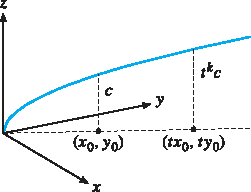
\includegraphics[width=0.4\paperwidth]{along_a_ray}
			\caption{Función $f$ a lo largo de un rayo.}\label{fig:along}
		\end{figure}
	\end{minipage}
\end{frame}

\begin{frame}
	\frametitle{\subsecname}
	\begin{minipage}{0.45\textwidth}
		En particular, sea $k=1$, así que $f\left(x,y\right)$ es homogénea de grado $1$. La curva $z=t^{k}c$ acostada verticalmente hacia arriba sobre cada rayo que pasa por el origen, es entonces la recta $z=tc$. Debido a esto, a menudo se dice que el \emph{gráfico de una función homogénea de grado} $1$ es generado por rectas que pasan por el origen. La figura~\ref{fig:homogenous} ilustra esto.
	\end{minipage}
	\begin{minipage}{0.45\textwidth}
		\begin{figure}
			\centering
			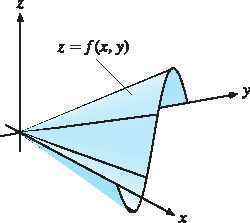
\includegraphics[width=0.4\paperwidth]{homogenous}
			\caption{$f$ es homogénea de grado $1$.}\label{fig:homogenous}
		\end{figure}
	\end{minipage}
\end{frame}


\begin{frame}[t]
\frametitle{\subsecname}
Hemos visto cómo, para una función $f\left(x,y\right)$ de dos variables, es a menudo conveniente considerar sus curvas de nivel en el plano $xy$ en vez de su gráfica tridimensional.

\

¿Qué podemos decir sobre las curvas de nivel de una función homogénea?

\

Resulta que \emph{para una función homogénea, incluso si solo se conoce sus curvas de nivel, también lo son sus otras curvas de nivel}. Para ver esto, considere una función $f\left(x,y\right)$ que es homogénea de grado $k$, y sea $f\left(x,y\right)=c$ una de sus curvas de nivel, como se ilustra en la figura~\ref{fig:levelcurves}.
\end{frame}

\begin{frame}
	\frametitle{\subsecname}
	\begin{minipage}{0.45\textwidth}
		Ahora explicamos cómo construir la curva de nivel que pasa un por un punto arbitrario $A$ no acostado en $f\left(x,y\right)=c$ en un punto $D$ con coordenadas $\left(x_{1},y_{1}\right)$. Las coordenadas de $A$ tendrán la forma $\left(tx_{1},ty_{1}\right)$ para algún valor de $t$ que en la figura es alrededor de $1.7$.
	\end{minipage}
	\begin{minipage}{0.45\textwidth}
		\begin{figure}
			\centering
			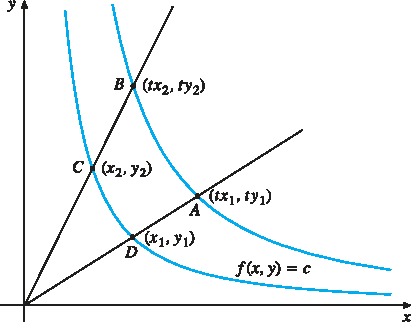
\includegraphics[width=0.4\paperwidth]{levelcurves}
			\caption{Curvas de nivel de una función homogénea.}\label{fig:levelcurves}
		\end{figure}
	\end{minipage}
\end{frame}

\begin{frame}[t]
\frametitle{\subsecname}
Con el fin de construir un nuevo punto en la misma curva de nivel como $A$, dibuje un nuevo rayo pasando por el origen. Suponga que este rayo intersecta la curva de nivel original $f\left(x,y\right)=c$ en $\left(x_{2},y_{2}\right)$. Ahora use el valor de $t$ encontrado antes para determinar el nuevo punto $B$ con coordenadas $\left(tx_{2},ty_{2}\right)$. Ahora este nuevo punto $B$ en la misma curva de nivel como $A$ debido a que $f\left(tx_{2},ty_{2}\right)=t^{k}f\left(x_{2},y_{2}\right)=t^{k}c=t^{k}f\left(x_{1},y_{1}\right)=f\left(tx_{1},ty_{1}\right)$. Repitiendo esta construcción para diferentes rayos a través del origen que intersecta la curva de nivel $f\left(x,y\right)=c$, podemos encontrar tantos punto como deseemos en la nueva curva de nivel $f\left(x,y\right)=f\left(tx_{1},ty_{1}\right)$.

El procedimiento argumentado muestra que una función homogénea $f\left(x,y\right)$ está completamente determinada por cualquiera de sus curvas de nivel y por su grado de homogeneidad. La forma de cada curva de nivel de una función homogénea es con frecuencia determinado especificando sus elasticidades de sustitución.
\end{frame}

\begin{frame}[t]
\frametitle{\subsecname}
Otro punto que vale la pena notar en relación con la figura~\ref{fig:levelcurves} es que las tangentes a las curvas de nivel a lo largo de cada rayo son paralelas. Mantenemos el supuesto que $f$ es homogénea de grado $k$. Si la curva de nivel es $f\left(x,y\right)=c$, su pendiente en el punto $\left(x,y\right)$ es $-f^{\prime}_{1}\left(x,y\right)/f^{\prime}_{2}\left(x,y\right)$. En el punto $A$ en la figura 12.6.3 la pendiente es
\begin{equation}
-\frac{f^{\prime}_{1}\left(tx_{1},ty_{1}\right)}{f^{\prime}_{2}\left(tx_{1},ty_{1}\right)}=-\frac{t^{k-1}f^{\prime}_{1}\left(x_{1},y_{1}\right)}{t^{k-1}f^{\prime}_{2}\left(x_{1},y_{1}\right)}=-\frac{f^{\prime}_{1}\left(x_{1},y_{1}\right)}{f^{\prime}_{2}\left(x_{1},y_{1}\right)}\tag{*}
\end{equation}
donde hemos usado la ecuación (12.6.3), expresando el hecho que las derivadas parciales de $f$ son homogéneas de grado $k-1$.

\	

Las igualdades en (*) establecen que dos curvas de nivel pasando por $A$ y $D$ tiene las mismas pendientes en esos puntos. Se sigue que, en cualquier punto a largo de un rayo pasando por el origen, la pendiente de la curva de nivel correspondiente muestra que es la misma. Declarado de manera diferente, después de quitar los signos menos, (*) muestra que la tasa marginal de sustitución de $y$ por $x$ es una función homogénea de grado $0$.
\end{frame}

\subsection{Funciones homogéneas y homotéticas}

\begin{frame}[t]
\frametitle{\subsecname}
Suponga que $f$ es una función de $n$ variables definida en su domino $D$. El conjunto $D$ es llamado un \emph{cono} si, cuando $\left(x_{1},x_{2},\ldots,x_{n}\right)\in D$ y $t>0$, el punto $\left(tx_{1},tx_{2},\ldots,tx_{n}\right)$ también se encuentra en $D$. Cuando $D$ es un cono, diremos que la función $f$ es \emph{homogénea de grado} $k$ \emph{en} $D$ si
\begin{equation}\label{eq:homogenea}
f\left(tx_{1},tx_{2},\ldots,tx_{n}\right)=t^{k}f\left(x_{1},x_{2},\ldots,x_{n}\right)
\end{equation}
para todo $t>0$. La constante $k$ puede ser cualquier número real, positivo, cero o negativo.
\begin{theorem}
	Suponga que $f$ es una función diferenciable de $n$ variables, definida en un cono abierto $D$. Entonces, $f$ es homogénea de grado $k$ si, y solo si, la siguiente ecuación se cumple para todo $\bm{x}$ en $D$:
	\begin{equation}\label{eq:euler}
	\sum_{i=1}^{n}x_{i}f^{\prime}_{i}\left(\bm{x}\right)=kf\left(\bm{x}\right)
	\end{equation}
\end{theorem}
La prueba de este resultado no es difícil, y complementa el argumento dado por el teorema 12.6.1:

\end{frame}

\begin{frame}[t]
\frametitle{\subsecname}

\begin{proofs}
Suponga que $f$ es homogénea de grado $k$, así satisface la ecuación~\eqref{eq:homogenea}. Diferenciando esta ecuación con respecto a $t$, cuando $\bm{x}$ es fijado, resulta \[ \sum_{i=1}^{n}x_{i}f^{\prime}_{i}\left(t\bm{x}\right)=kt^{k-1}f\left(\bm{x}\right). \] Haciendo $t=1$ da~\eqref{eq:euler} inmediatamente.

Para probar la recíproca, asuma que la ecuación~\eqref{eq:euler} es válida para cualquier $\bm{x}$ en el cono $D$. Mantenga $\bm{x}$ fijado y defina la función $g$ para todo $t>0$ por $g\left(t\right)=t^{-k}f\left(t\bm{x}\right)-f\left(\bm{x}\right)$.
\end{proofs}

\end{frame}
% TODO: Ver 1307.3973.pdf para la geometría de la función ACMS.
% TODO: Ver los gráficos 1907.12624.pdf
% TODO: Ver las clases de equivalencias en Copulas
% TODO: Usaste el artículo de Arrow para las deducciones de 
\begin{frame}[t]
\frametitle{\subsecname}
\begin{proofs}[\proofname\ (Cont.)]
 Entonces, diferenciando da
\begin{equation}
g^{\prime}\left(t\right)=-kt^{-k-1}f\left(t\bm{x}\right)+t^{-k}\sum_{i=1}^{n}x_{i}f^{\prime}_{i}\left(t\bm{x}\right).
\end{equation}
Debido a que $t\bm{x}$ se encuentra en $D$, la ecuación~\eqref{eq:euler} también debe ser válida cuando cada $x_{i}$ es reemplazada por $tx_{i}$. Se sigue que $\sum_{i=1}^{n}\left(tx_{i}\right)f^{\prime}_{i}\left(t\bm{x}\right)=kf\left(t\bm{x}\right)$.

\

Multiplicando esta ecuación por $t^{-k-1}$ y usando esto para sustituir por el último término de (*) implica que, para cualquier $t>0$, uno tiene \[ g^{\prime}\left(t\right)=-kt^{-k-1}f\left(t\bm{x}\right)+t^{-k-1}kf\left(t\bm{x}\right)=0. \] Se sigue que $g\left(t\right)$ debe ser una constante $C$. Obviamente, $g\left(1\right)=0$, así que $C=0$, lo que implica que $g\left(t\right)=0$ para todo $t>0$. De acuerdo con la definición de $g$, esto prueba que $f\left(t\bm{x}\right)=t^{k}f\left(\bm{x}\right)$, así que $f$ en realidad es homogénea de grado $k$.
\end{proofs}
\end{frame}

\begin{frame}[t]
\frametitle{\subsecname}
Una versión interesante de la ecuación de Euler, ecuación~\eqref{eq:euler}, es obtenida dividiendo cada término de la ecuación por $f\left(f\left(\bm{x}\right)\right)$, dado que este número no es $0$. Recordando la definición de la elasticidad paricial, $\operatorname{El}_{i}f\left(\bm{x}\right)=\left(\frac{x_{i}}{f\left(\bm{x}\right)}\right)f^{\prime}_{i}\left(\bm{x}\right)$, tenemos
\begin{equation}
\operatorname{El}_{1}f\left(\bm{x}\right)+\operatorname{El}_{2}f\left(\bm{x}\right)+\cdots+\operatorname{El}_{n}f\left(\bm{x}\right)=k
\end{equation}
Así, la suma de las elasticidades parciales de una función de $n$ variables que es homogénea de grado $k$ debe ser igual a $k$.

\begin{definition}
Sea $f$ una función de $n$ variables $\bm{x}=\left(x_{1},\ldots,x_{n}\right)$ definida en un cono $K$. Entonces, $f$ es llamada \emph{homotética} si \[ \forall\bm{x},\bm{y}\in K,f\left(\bm{x}\right)=f\left(\bm{y}\right),t>0\implies f\left(t\bm{x}\right)=f\left(t\bm{y}\right). \]
\end{definition}
\end{frame}